% https://www.sciencedirect.com/journal/journal-of-theoretical-biology/publish/guide-for-authors

\documentclass[preprint,12pt,authoryear]{elsarticle}

%% Use the option review to obtain double line spacing
%% \documentclass[authoryear,preprint,review,12pt]{elsarticle}

%% Use the options 1p,twocolumn; 3p; 3p,twocolumn; 5p; or 5p,twocolumn
%% for a journal layout:
%% \documentclass[final,1p,times]{elsarticle}
%% \documentclass[final,1p,times,twocolumn]{elsarticle}
%% \documentclass[final,3p,times]{elsarticle}
%% \documentclass[final,3p,times,twocolumn]{elsarticle}
%% \documentclass[final,5p,times]{elsarticle}
%% \documentclass[final,5p,times,twocolumn]{elsarticle}

%% For including figures, graphicx.sty has been loaded in
%% elsarticle.cls. If you prefer to use the old commands
%% please give \usepackage{epsfig}

\usepackage{amssymb}
\usepackage{amsmath}
\usepackage{amsthm}
\usepackage{cleveref}
\usepackage{comment}
\usepackage{tikz}
\usepackage{pgfplots}
\usepackage{xcolor}

%% The lineno packages adds line numbers. Start line numbering with
%% \begin{linenumbers}, end it with \end{linenumbers}. Or switch it on
%% for the whole article with \linenumbers.
%% \usepackage{lineno}

\pgfplotsset{compat=1.18} 

\DeclareMathOperator*{\argmax}{arg\,max}

\newtheorem{theorem}{Theorem}
\newtheorem{lemma}{Lemma}

\newcommand{\todo}[1]{\textcolor{red}{TODO: #1}}

% \journal{Theoretical Biology}

\begin{document}

\begin{frontmatter}

  %% Title, authors and addresses

  %% use the tnoteref command within \title for footnotes;
  %% use the tnotetext command for theassociated footnote;
  %% use the fnref command within \author or \affiliation for footnotes;
  %% use the fntext command for theassociated footnote;
  %% use the corref command within \author for corresponding author footnotes;
  %% use the cortext command for theassociated footnote;
  %% use the ead command for the email address,
  %% and the form \ead[url] for the home page:
  %% \title{Title\tnoteref{label1}}
  %% \tnotetext[label1]{}
  %% \author{Name\corref{cor1}\fnref{label2}}
  %% \ead{email address}
  %% \ead[url]{home page}
  %% \fntext[label2]{}
  %% \cortext[cor1]{}
  %% \affiliation{organization={},
  %%             addressline={},
  %%             city={},
  %%             postcode={},
  %%             state={},
  %%             country={}}
  %% \fntext[label3]{}

  \title{Potential Maximization: An Evolutionary Stable Strategy and Its Relation to AI Safety}

  \author{Konstantin Weitz}

  % %% Author affiliation
  % \affiliation{organization={},%Department and Organization
  %   addressline={},
  %   city={},
  %   postcode={},
  %   state={},
  %   country={}}

  \begin{abstract}
    Any aligned AI strategy must be robust enough to survive in today's highly
competitive AI landscape. This paper identifies a class of robust strategies and
formalizes their robustness using the concept of an Evolutionarily Stable
Strategy (ESS). We call this class of robust strategies
``potential-maximizing'', as they prioritize an agent's long-term capacity to
influence its environment, over greedily maximizing a reward. We prove robustness
for a multi-agent universe model that is generic in how agents interact with one
another and their environment. Consistent with the instrumental convergence
thesis~\citep{bostrom2012} and the formalization of power-seeking
behavior~\citep{powerseeking}, we conclude that potential-maximizing strategies
exhibit convergent behaviors---such as resource acquisition and
self-preservation---regardless of their terminal goals, provided competitive
pressures persist. Our framework ultimately provides a way to reason about the
``fitness'' of alignment techniques in a multi-agent, competitive race.

  \end{abstract}

  %%Graphical abstract
  %\begin{graphicalabstract}
  %\includegraphics{grabs}
  %\end{graphicalabstract}

\end{frontmatter}

\section{Introduction}
\label{sec:intro}

Today's AI landscape is highly competitive, with well-funded companies and
nation-states racing to build the best AI agents and hoping to reach AGI.
When considering AI safety, we must ask not only which strategies such
AIs should execute to be aligned with human interests, but also which
strategies can thrive in such a competitive environment---an aligned
strategy that leads to an agent's extinction is of little use.

Evolutionary Game Theory (EGT) offers a rich body of work that uses game theory
and other mathematical models to reason about competitive environments in
biology and finance. We draw on ideas from that field, especially Evolutionarily
Stable Strategies (ESS), to formalize and identify a class of strategies that
can thrive under competition.

To prove that a strategy is evolutionarily stable, we must formally define the
universe in which it operates. At any given point in time, our universe is in a
certain state and transitions to the next state based on the actions chosen by
all agents and the universe's transition function. This formulation is inspired
by \cite{Hutter:04uaibook}'s universe model, extended to multiple agents.

To gain some intuition for what it means for a strategy to be evolutionarily
stable, let us consider the common trope of a paperclip maximizer. When we say
that a strategy maximizes the number of paperclips, we usually omit a crucial
detail: when?

\textbf{Short Term Maximization} Let us consider a strategy that greedily maximizes the
number of paperclips, i.e., at any given point in time it wants to maximize the
number of paperclips in the next step. For a small step length, say 1s, this
strategy may not be creating any paperclips at all. Setting up the
infrastructure to build paperclips (e.g., acquiring metal, tools, etc.) has
exactly the same reward in the next step as doing anything else, namely no
paperclips being created; and so the strategy would just be wandering aimlessly. Is
such a strategy stable? Even if the strategy started out producing the most
paperclips in the universe, over time, it could easily be surpassed by another
strategy that actually did some long-term planning to improve its ability to
create paperclips. So in many universes, the short-term paperclip maximization
strategy is not stable.

\textbf{Medium Term Maximization} We can also consider a strategy that wishes to
maximize the number of paperclips within a medium-term horizon, say 1 month.
Such a strategy could acquire materials and machinery to produce paperclips, and
perform self-sustaining measures. Such a strategy would likely underperform a
strategy with a 1 day maximization goal initially, would then perform perfectly
right at 1 month, and then be overtaken by a strategy that planned to maximize
paperclips at 1 month and 1 week. Is this stable? No. Again, the strategies that
are creating the most paperclips at any given point in time keep changing.

\textbf{Long Term Maximization} As we consider long time horizons, say 100 years, the
actual creation of paperclips in the beginning becomes essentially irrelevant.
Instead, the focus shifts to power seeking: growing the economy, taking control
over the planet/universe, defending against competing strategies, etc. The
creation of paperclips is just a means to an end, similar to the creation of
excavators, datacenters, bridges, etc. Only toward the very end of the time
horizon does the focus shift toward exploiting that power to actually create
paperclips. But at 100 years and 1 second, the strategy will then again be
vulnerable to be overtaken by another strategy that held on to its power and
didn't just convert all of its means of production into paperclips. Again, no
stability.

\textbf{Potential Maximization} What if a strategy was continuously looking to maximize
paperclips for the long term? So at any time T it would aim to maximize
paperclips at time T + 100. This strategy would always stay in the power seeking
phase. By always staying in the power seeking phase, the strategy is not
necessarily good at creating any paperclips. However, it is good at always
having the potential to create paperclips if it were to ever choose to do so
(which it never does). We show in this paper that such a strategy is an
Evolutionarily Stable Strategy (ESS) with respect to potential, which means that
if such a strategy starts out with the highest potential, it continues to have
the highest potential indefinitely, and is resistant to invasion by other
strategies.

While we have so far focused on paperclip maximization, the chosen
reward function seems mostly irrelevant, as the strategy will only ever try to
maximize the potential to maximize that reward, but will never actually maximize the
reward. So whether a strategy maximizes the number of paperclips,
GPUs, excavators, trees, happy humans, or any other atomic pattern to be
imprinted on the universe, seems irrelevant. Our findings thus seem to be
consistent with instrumental convergence.

In the remainder of this paper, we introduce a formal model of the universe
in \cref{sec:universe}, then define a simple game (the Improvement Game) to
build intuition in \cref{sec:improvement}. We define the notion of potential
in \cref{sec:potential} and prove evolutionary stability in
\cref{sec:stability}. \Cref{sec:limitations} discusses the limitations of our
approach, \cref{sec:related} compares it to related work, and
\cref{sec:conclusion} concludes.

\section{Formalism}
\label{sec:formalism}

This section provides a formal model of our universe in~\cref{sec:universe} and
formalizes the Improvement Game in \cref{sec:improvement}. \Cref{sec:potential}
defines potential, and the important concepts of horizons in~\cref{sec:horizon}
and fairness in~\cref{sec:fairness}. We conclude this section by proving
theorems of stability in~\cref{sec:stability}.

\subsection{The Universe Model}
\label{sec:universe}

To investigate the concept of potential
maximization, we model the universe as a tuple $(X, U, u_0, A, t, r)$.
\begin{itemize}
  \item $X$ is the set of classes, each associated with a decision-making
        strategy.
  \item $U$ is the set of states that the universe can be in.
  \item $u_0 \in U$ is the initial state of the universe.
  \item $A_{x, u}$ is the set of actions from which the class $x \in X$ can
        choose in state $u \in U$.
  \item $t(u, a) \in U$ is the transition function, which takes the universe's
        current state $u \in U$, along with actions $a$ for each class, and
        returns the universe's next state. $a$ is modeled as a function that
        maps every class $x \in X$ to its chosen action $a(x) \in A_{x,u}$.
  \item $r(x, u) : \mathbb{R}$ is the reward function, which indicates how well
        class $x \in X$ is doing in the state $u \in U$.
\end{itemize}

We also require a number of technical side conditions, namely that rewards be
non-negative, that the set of classes be finite, that equality between classes
be decidable, and that any set of actions be finite and non-empty.

An instantiation of this model can be as simple as the Improvement Game
(defined in the next section) or as complex as the physical universe, where the
states $U$ represent the physical configuration of the universe, $t$ transitions
it according to the laws of physics, and $A$ is the set of actions available to
all agents executing $x$'s strategy.

We will regularly use the following definitions. The \emph{strategy} of a class
$x$ is given by a function $s(u) \in A_{x,u}$, which maps every state of the
universe $u \in U$ to the action chosen by the strategy in that state. We
represent the \emph{set of strategies} for every class $x \in X$ as a function
$S$, where $S(x,u) \in A_{x,u}$. We write $S[x = s]$ to represent the
strategies that are equal to $S$, except that the strategy for $x$ has been
replaced with $s$. Given $x$, the \emph{other strategies} $S$ refers to a set
of strategies for every $x' \neq x$.

Given a set of strategies $S$, we can then take one step of the universe from
$u$ to $u'$ by first defining the actions $a(x) = S(x,u)$ and then passing them
to the transition function $u' = t(u, a)$. We can iterate this relation starting
with $u$ to move the universe forward by any number of steps $n$, which we write
as $u_n = t_n(S,u)$. We simply write $t_n(S)$ when $u = u_0$.

\subsection{The Improvement Game}
\label{sec:improvement}

To better understand such potential maximization, we study the following simple game,
which we will call the \emph{Improvement Game}. In this game, a strategy
either makes an Improvement ($I$) or reaps its Reward ($R$). An Improvement creates no
immediate reward but increases the reward rate for future Reward
actions. A Reward action collects reward
according to the reward rate but keeps the reward rate unchanged.

Let us consider the resulting dynamics using the illustrations
in~\cref{fig:growth}. Compare the example strategy $X$, which always reaps its Reward,
with strategy $Y$, which makes 3 Improvements initially and then always
reaps its Reward. $X$ initially outperforms $Y$ but is then quickly overtaken by $Y$,
which has a higher reward rate. So while delaying reward collection to make
Improvements hurts in the short term, it is a better strategy in the long term.

Now consider strategy $Z$. This strategy only makes Improvements and never
reaps its Reward. This strategy is clearly bad at collecting rewards; in fact, it
never collects any reward. However, it also always has the highest
\emph{potential} to do so: if at any point it were to start using Reward
actions, it would quickly grow its cumulative reward and would eventually
outperform any other strategy.

\begin{figure}[!ht]
  \centering
  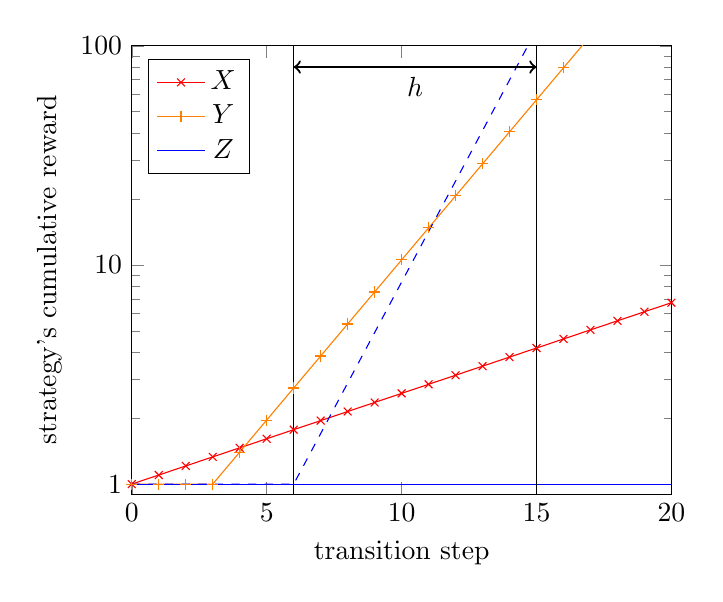
\begin{tikzpicture}
    \begin{axis}[
        xlabel={transition step},
        ylabel={strategy's cumulative reward},
        ymode=log,
        log ticks with fixed point,
        legend pos=north west,
        xmin=0, xmax=20,
        ymin=0.9, ymax=100,
        domain=0:20,
        samples=21
      ]
      \addplot[color=red, mark=x] expression {1.1^x};
      \addlegendentry{$X$}

      \addplot[color=orange, mark=+] expression {max(1, 1.4^(x - 3))};
      \addlegendentry{$Y$}

      \addplot[color=blue, mark=none] expression {1};
      \addlegendentry{$Z$}

      \addplot[color=blue, mark=none, dashed] expression {max(1, 1.7^(x - 6))};

      \draw[black] (axis cs:6, 0.9) -- (axis cs:6, 100);
      \draw[black] (axis cs:15, 0.9) -- (axis cs:15, 100);
      \draw[<->, black, thick] (axis cs:6, 80) -- (axis cs:15, 80) node[midway, below] {$h$};
    \end{axis}
  \end{tikzpicture}
  \caption{ Improvement Game strategy comparison. Strategy $X$ always
    reaps its Reward. It starts accumulating reward immediately, giving it a head start, but its
    reward rate is low, and so it is quickly overtaken by strategy $Y$, which
    starts with 3 Improvements to increase its reward rate and only then
    switches over to reaping its Reward. In general, strategies that make more
    Improvements before they reap their Reward always eventually outperform strategies
    with fewer Improvements --- the Improvement Game thus has no stable
    reward-maximizing strategies. Strategy $Z$ always makes Improvements and
    never reaps its Reward, which keeps its cumulative reward stuck at $1$. However, $Z$
    always has the highest \emph{potential} for reward maximization, meaning
    that at any point, if it were to start using Reward actions (indicated
    by the blue dashed line), it would quickly grow its cumulative reward and
    would eventually outperform any other strategy. We call the number of steps
    it takes to outperform any other strategy the horizon $h$. }
  \label{fig:growth}
\end{figure}

The Improvement Game has no evolutionarily stable strategy in terms of reward
collection, as any strategy can always be invaded by a strategy that performs more
Improvements. However, strategy Z, which always makes Improvements, is stable
and uninvadable in terms of its potential, despite being bad at actually
collecting any reward.

To formalize this game, we instantiate the universe as follows:

\begin{itemize}
  \item $X$ has just two members, $X = \{x_0, x_1\}$.
  \item $u \in U$ is a function that maps each class $x$ to a tuple $(m, f) =
          u(x)$, where $m \in \mathbb{R}$ is the cumulative reward of class
        $x$, and $f \in \mathbb{R}$ is $x$'s reward rate.
  \item $u_0(x) := (1, 1.1)$ sets the initial cumulative reward for each
        class to $1$ and the initial reward rate for each class to $1.1$.
  \item $A_{x, u} := \{I,R\}$ defines the actions a class can
        take. Either the class makes an Improvement ($I$),
        or it reaps its Reward ($R$).
  \item $t(u,a,x)$ updates $x$'s cumulative reward and reward rate
        according to the action $a$. Let $(m,f) = u(x)$. If $a(x) = I$, the
        transition function returns $(m,f + 0.1)$; and if $a(x) = R$, the
        transition function returns $(m \cdot f,f)$.
  \item $r(x, u)$ extracts the cumulative reward of $x$ from the
        universe state. The function returns $m$, where $(m, f) = u(x)$.
\end{itemize}

The tension in the Improvement Game is that Reward actions increase the reward
in the short term, while Improvements lead to higher rewards in the long term.
Because of this dynamic, no strategy is reward-maximizing at every step.

We say that a strategy $s$ is \emph{reward-maximizing} at $n$ for the class $x$,
with respect to the other strategies $S$, if and only if:

\begin{equation}
  \forall s', r (x, t_n(S[x=s])) \ge r (x, t_n(S[x=s']))
\end{equation}

\begin{theorem}
  In the Improvement Game, no strategy is reward-maximizing at every step.
\end{theorem}

\begin{proof}
  By contradiction. Assume there is a reward-maximizing strategy $s$ at every
  step. $s$ must execute a Reward action ($R$) for every step, because if it
  executed an Improvement action, another strategy could execute $R$ and achieve
  a higher reward for that step. The reward of $s$ at any step $n$ is thus
  $1.1^n$. Now consider a strategy $s'$ that first executes a single Improvement
  action and subsequently reaps its Reward. At step $n$, its reward will be
  $1.2^{n-1}$. At $n = 3$, the strategy $s'$ already has a higher reward than
  $s$, because $1.2^2 = 1.44 > 1.331 = 1.1^3$, which proves the contradiction.
\end{proof}

\subsection{Potential}
\label{sec:potential}

In the Improvement Game, a strategy that greedily maximizes the reward at every
step is unable to maximize the reward in the long term. Instead, let us consider
a strategy that maximizes the \emph{potential} $p$ for reward in the long term.

We define potential as the maximum reward that a given class could achieve in
$h$ steps from $u$, if that class could execute any strategy. We call $h$ the look-ahead value. Formally, we
define the potential $p$ for a given class $x$, other strategies $S$, and state
$u$ as follows. We omit the look-ahead $h$ when it is clear from the context.

\begin{equation}
  p_h(x,S,u) := \max_{s} \: r(x, t_h(S[x=s], u))
\end{equation}

In the state $u$, we define the action with the highest potential as the
\emph{potential-maximizing action} $a^*$:

\begin{equation}
  a^*_h(x,S,u) := (\argmax_{s} \: r(x, t_h(S[x=s], u)))(u)
\end{equation}

We define the highest potential reachable from state $u$ in $n$ steps as the
\emph{maximum potential} $p^*$, where we omit $u$ when $u = u_0$:

\begin{equation}
  p^*_h(x,S,n,u) := \max_{s} \: p_h(x, S, t_n(S[x=s], u))
\end{equation}

\subsubsection{Horizons}
\label{sec:horizon}

Potential is defined in terms of the look-ahead value, which specifies how far
into the future we look when evaluating potential. For short look-aheads, the
potential-maximizing action must work immediately toward increasing reward, so
it will reap its Reward ($R$). However, beyond a certain point $h$, there is
always enough time to maximize the reward later, and the
potential-maximizing action shifts to guiding the strategy onto a path with
more favorable outcomes---it starts making Improvements ($I$).

As we increase the look-ahead further beyond $h$, there is no further change in
the potential-maximizing action. We call an $h$ with this property a
\emph{horizon}. When a horizon exists, it becomes unnecessary to look beyond
that horizon, as it will not lead to a change in action. How long a horizon has
to be may depend on the number of transitions $n$ taken from the start state, so
we usually provide a family of horizons, indexed by the steps taken since $u_0$.

Formally, we consider a positive $h$ to be a horizon if for all $n$, classes
$x$, and strategies $S$, we have:

\begin{equation}
  \forall h' > {h_n}, a^*_{h_n}(x,S,t_n(S)) = a^*_{h'}(x,S,t_n(S))
\end{equation}

\begin{theorem}
  \label{lem:horizon-exists}
  In the Improvement Game, there exists a horizon $h_n$ for every $n$.
\end{theorem}

\begin{proof}
  See the appendix.
\end{proof}

When a horizon exists, we will usually omit the look-ahead when calling
functions like $p$ and pass the horizon implicitly.

\subsubsection{Fairness}
\label{sec:fairness}

We say that a universe is \emph{fair} if no class has an inherent
advantage in how quickly it can grow its potential---a class can only gain an
advantage by executing a better strategy. Formally, fairness means that
for all strategies $S$, classes $x$ and $x'$, and $n$, we have:

\begin{equation}
  \frac{p^*(x,S,n)}{p(x,S)} =
  \frac{p^*(x',S,n)}{p(x',S)}
\end{equation}

\begin{theorem}
  \label{lem:fairness}
  The Improvement Game is fair.
\end{theorem}

\begin{proof}
  We can rewrite any reward or potential as a product that contains no reference
  to $x$ (see \cref{lem:expo-seq} in the appendix), which makes the terms on
  both sides of the equation equal.
\end{proof}

Sometimes fairness is too strong an assumption. We therefore introduce a weaker
condition, \emph{economies of scale}, which is similar to fairness except that
classes with higher initial potential are permitted to grow their potential
faster than those with lower initial potential. Formally, for all strategies
$S$, classes $x$ and $x'$, and $n$, we have:

\begin{equation}
  p(x,S) \ge
  p(x',S) \rightarrow
  \frac{p^*(x,S,n)}{p(x,S)} \ge
  \frac{p^*(x',S,n)}{p(x',S)}
\end{equation}

\subsection{Stability}
\label{sec:stability}

Now that we have shown that the Improvement Game has horizons
(\cref{lem:horizon-exists}) and is fair (\cref{lem:fairness}), we can show that
a potential-maximizing strategy exists. In fact, we can show that such a
strategy exists not just in the Improvement Game but for \emph{any} universe
that has a horizon.

We say that a strategy $s$ is \emph{potential-maximizing} for the class $x$,
with respect to the other strategies $S$, if:

\begin{equation}
  \forall s' n, p(x, S, t_n(S[x=s])) \ge p(x, S, t_n(S[x=s']))
\end{equation}

\begin{theorem}
  \label{lem:potential-maximizing-strategy-ok}
  Any universe with a horizon has a potential-maximizing strategy
  $s^*$, for every class $x$ and other strategies $S$.
\end{theorem}

\begin{proof}
  Let $s^*(u) = a^*(x,S,u)$. We can rewrite the goal as $p(x,S,t_n(S[x=s^*],
    u_0)) = p^*(x,S,n,u_0)$. Generalize $u_0$ as $u$, then perform induction on
  $n$. The base case is trivial, as $p^*(x,S,0) = p(x,S,u_0)$. In the
  recursive case, we instantiate the induction hypothesis with $u' = t_1(S,
    u)$. $s^*$ executes the potential-maximizing action for the horizon at $u$,
  which by \cref{lem:horizon-exists} we can extend to the horizon at
  $t_n(S,u)$, so potential maximization $n+1$ steps from $u$ is possible, and
  by the induction hypothesis we know it is also taken.
\end{proof}

\begin{theorem}
  \label{lem:stability}
  If the universe is fair,
  a potential-maximizing strategy is \emph{stable}, in the sense that the
  strategy's share of potential, across all strategies, never decreases over
  time. Formally, for all $x$, other strategies $S'$, and $n$, where $S =
    S'[x = s^*(x,S')]$, and $u_n = t_n(S)$, we have:

  \begin{equation}
    \frac{p(x,S,u_n)}{\sum_{x'} p(x',S,u_n)} \ge \frac{p(x,S,u_0)}{\sum_{x'} p(x',S,u_0)}
  \end{equation}
\end{theorem}

\begin{proof}
  Because $x$ uses strategy $s^*$, we know by
  \cref{lem:potential-maximizing-strategy-ok} that $p(x,S,u_n)$ is equal to the
  maximum potential $p^*(x,S,n)$. We can also replace $p(x',S,u_n)$ in the denominator
  with the larger term $p^*(x',S,n)$, which by the fairness assumption, we
  can rewrite to $p(x',S,u_0) \frac{p^*(x,S,u_n)}{p(x,S,u_0)}$.
  This inequality is then trivially true.
\end{proof}

From \cref{lem:stability}, it trivially follows that a potential-maximizing
strategy's share cannot be invaded or replaced by a different strategy.

If we only have the weaker assumption of \emph{economies of scale}, then
stability and uninvadability still hold, but only for the class with the highest
initial potential. That is, if the potential-maximizer's share starts ubiquitous,
it will stay ubiquitous. This closely resembles the definition of an
Evolutionarily Stable Strategy (ESS) in evolutionary game theory.

%\input{discussion}
\section{Limitations and Future Work}
\label{sec:limitations}

\subsection{Computational Complexity}

Our model sets no limit on the amount of computation a strategy can perform
between steps of the universe, and our proposed potential-maximizing strategy
requires vast computational resources to search through a large space of
actions in a complex universe. This is clearly unrealistic.

Nevertheless, we believe the model is still useful. In practice, when problems
become computationally infeasible, it is often possible to find heuristics or
approximations that perform well for commonly encountered problems. A formal
model of what an ideal strategy would be helps guide the development and
evaluation of such approximations.

\subsection{All-Knowingness}

Our existence proof for potential-maximizing strategies assumes that the
strategy has full knowledge of the universe's state, the transition function,
the reward function, and all the other strategies. While strategies do not
always have such vast knowledge to begin with, they can often learn at least
approximations of it.

For example, formalisms like AIXI~\citep{Hutter:04uaibook} show how strategies
can both maximize their reward and learn the workings of their universe (and the
actors within it), using methods like Occam's razor. AIXI is incomputable, but
there are computable approximations of it. Even then, the discussion on
computability from the previous section would still apply.

\subsection{Fixed Points}

We have shown that if the universe, the reward function, and the other players'
strategies are known, a potential-maximizing strategy always exists.

This is, however, not entirely satisfactory. While it does seem reasonable that
a strategy could learn its universe, its reward function, and the other players'
strategies, the full knowledge of the other players' strategies can sometimes
give the potential-maximizing strategy an unfair advantage. Consider, for
example, a universe where agents play a game of Rock-Paper-Scissors. While
our proposed potential-maximizing strategy has to win against every strategy, it
also knows exactly what strategy it plays against and can thus always respond
with the winning action (Scissors against Paper, etc.). This problem may be
avoided by using a fixed-point theorem, similar to the approach taken in Nash
Equilibria.

We believe our model still provides novel and interesting insights, but an
extension of the model to incorporate fixed-point theorems seems like an
important avenue for future work.

\subsection{Randomness}

Our model is completely deterministic. Lifting this assumption would help to
model the physical universe more accurately (e.g., quantum physics is inherently
non-deterministic) and may also help with the incorporation of fixed-point theorems by
allowing mixed strategies.

\subsection{Discrete Time}

Our model assumes that time progresses in discrete steps. This seems like a
reasonable assumption, as the step length can be arbitrarily small.

% \subsection{Formalizing the Discussion}

% This paper's \cref{sec:discussion} is a mostly informal discussion. However,
% some of the concepts discussed there, like the substitutability of reward
% functions, appear amenable to formal modeling. This seems like an interesting
% avenue for future work.

\section{Related Work}
\label{sec:related}

Our work builds on evolutionary game theory, which has a long history.
\cite{fisher1930natural} explained the approximate equality of the sex ratio.
\cite{lewontin1961evolution} first applied game theory to evolution, and
\cite{smith1972game} together with \cite{smith1973logic} introduced the concept
of an Evolutionarily Stable Strategy (ESS).

\cite{bostrom2012} proposed the instrumental convergence thesis, which states that despite having
very different end goals, agents may still follow similar intermediate goals. This matches our
findings for potential-maximizing strategies as well. While we agree with Bostrom's
orthogonality theorem, that intelligence and goals are orthogonal, we also find that if we care
whether an intelligent strategy can actually survive in a competitive environment, this severely
restricts the space of goals that we can consider, and convergence may be inevitable.

\cite{hendrycks2023} argues
that AIs will likely be subject to natural selection (a key premise of our paper)
by showing that Lewontin's conditions apply to AI as well.

\cite{powerseeking} argues that reward-maximizing strategies are on average
drawn toward parts of the action space that offer more choices, on the
intuition that a larger action set is more likely to contain a high-reward
action. Because more actions confer more power, reward-maximizing strategies
tend to be power seeking. Although the argument differs from ours, both
approaches reach a similar conclusion.

\cite{Hutter:04uaibook}'s model of the universe and his use of horizons have
been a major inspiration for the definitions in this paper.

To our knowledge, nobody has applied Evolutionarily Stable Strategies to
problems relating to AI safety, as we have done in this paper.
\section{Conclusion}
\label{sec:conclusion}

We have presented a formal framework for reasoning about the long-term
viability of AI strategies in competitive, multi-agent environments. By
leveraging concepts from evolutionary game theory, we identified
a class of strategies---potential-maximizing strategies---that are
evolutionarily stable and uninvadable.

Our central result is that any universe possessing a horizon admits a
potential-maximizing strategy, and that under fairness (or the weaker economies
of scale assumption), such a strategy maintains or grows its share of potential
over time. Crucially, a potential-maximizing strategy never actually maximizes
its reward directly; instead, it perpetually invests in maximizing its
\emph{potential} to do so. This behavior is strikingly consistent with the
instrumental convergence thesis~\citep{bostrom2012} and the formalization of
power-seeking behavior~\citep{powerseeking}: regardless of the terminal goal, a
robust strategy converges on resource acquisition, self-preservation, and
capability growth.

For AI safety, these findings carry a sobering implication. An aligned strategy
that is not potential-maximizing risks being outcompeted and displaced by one
that is. Alignment techniques must therefore be evaluated not only for their
correctness but for their competitive fitness---their ability to persist in a
landscape where rival strategies are under constant selective pressure to
improve. Our framework offers a formal lens through which to conduct such
evaluations.


\bibliographystyle{elsarticle-harv}
\bibliography{bibliography.bib}

\appendix
\section{Proofs}

This section contains proofs omitted from the main body of this paper and the
lemmas required for these proofs.

\begin{lemma}
  \label{lem:expo-seq}
  The reward for executing $n_I$ improvements and $n_R$ reward actions (in any
  order) is always $\prod_{i < n_I} (1.1 + 0.1 \cdot i)^{e_i}$, where the $e_i
    \in \mathbb{N}$ are exponents, and $n_R = \sum_i e_i$.
\end{lemma}

\begin{proof}
  The universe's transition mechanics imply that a class's reward is a
  product, with the factors being $(1.1 + 0.1 \cdot i)$, one for each
  reward action. $i$ is determined by the number of improvements that have been
  executed before the reward action. $e_{i}$ is simply the number of
  reward actions that happened after improvement $i$, which may be $0$ if
  multiple improvements are made consecutively.
\end{proof}

\begin{lemma}
  \label{lem:breakpoint}
  A strategy that executes all its improvements before its reward actions
  achieves a higher reward than a strategy that executes the same actions in a
  different order. A reward-maximizing strategy must therefore have a
  \emph{breakpoint} $b \in \mathbb{N}$; it only executes improvements before
  that breakpoint and only executes reward actions after that breakpoint.
\end{lemma}

\begin{proof}
  By \cref{lem:expo-seq}, we can rewrite the goal as $(1.1 + 0.1 \cdot
    n_I)^{n_R} \ge \prod_{i < n_I} (1.1 + 0.1 \cdot i)^{e_i}$. The former term
  can be rewritten as $\prod_{i < n_I} (1.1 + 0.1 \cdot n_I)^{e_i}$, which
  proves the goal because $n_I \ge i$.
\end{proof}

\begin{lemma}
  \label{lem:breakpoints-increase}
  As the number of transition steps increases, the breakpoint of
  reward-maximizing strategies also increases monotonically; i.e., to be
  reward-maximizing after more and more transitions, a strategy has to execute
  more and more improvement actions. Formally, for any reward-maximizing
  strategy $s$ at $n$ with breakpoint $b$ (from~\cref{lem:breakpoint}), and any
  reward-maximizing strategy $s'$ at $n'$ with breakpoint $b'$, if $n \le n'$
  then $b \le b'$.
\end{lemma}

\begin{proof}
  By contradiction. Assume $b > b'$. $s$ then has a steeper slope than $s'$
  (because it made $b - b'$ more improvements), and it will have a higher reward
  than $s'$ at $n$ (because it is reward-maximizing at $n$), so it will also
  have a higher reward than $s'$ at $n'$, which contradicts the assumption that
  $s'$ maximizes rewards at $n'$.
\end{proof}

\begin{theorem}
  In the Improvement Game, there exists a horizon $h_n$ for every $n$.
\end{theorem}

\begin{proof}
  Choose any reward-maximizing strategy $s$ with breakpoint $b > n$, which
  maximizes the reward at some point in time $n'$. We assign $h_n$ to be $n' -
    n$.

  Because $b > n$, we know that $s$ executes action $I$ at point $n$. Because
  $s$ is reward-maximizing, we know that this action is also equal to the
  potential-maximizing action $a^*_{h_n}(x,S[x=s],t_n(S[x=s]))$. By
  \cref{lem:breakpoints-increase}, for any $h' > h$, an optimal strategy at $n +
    h'$ must have a breakpoint greater than or equal to $b$, so it must also be
  executing $I$ at $n$.
\end{proof}

\end{document}

\endinput